% slides-exemplo-beamer
%
% S�b Out  1 19:47:43 BRT 2011

\documentclass[table, usenames, svgnames, dvipsnames]{beamer}
\usepackage{beamerthemeshadow}
\usepackage[brazilian]{babel}
\usepackage[latin1]{inputenc}
\usepackage[absolute,overlay]{textpos}
\usepackage{array}

%\usepackage{subfigure}
%\usepackage{multicol}
%\usepackage{colortbl}

% ---------------------------------------------------------------------------- %
% Defini��es beamer
% ---------------------------------------------------------------------------- %
\usetheme{Rochester}
%\usetheme{Luebeck}
\usecolortheme{rose}

% Algumas defini��es para o layout
\setbeamerfont{frametitle}{size=\normalsize}
\setbeamerfont{title}{size=\normalsize}
\beamertemplatenavigationsymbolsempty

% Podem ser utilizadas imagens no background
%\setbeamercolor{frametitle}{bg=black}
%\usebackgroundtemplate{\includegraphics[height=\paperheight]{figuras/back.jpg}}

% Os simbolos de navegacao nao sao necessarios
\setbeamertemplate{navigation symbols}{}
\setbeamertemplate{footline}{}

%\setbeamertemplate{footline}[page number]{}
%\setbeamertemplate{footline}[text line]{ \hfill {\insertframenumber}}

% Indice para cada se��o (aparece antes de cada section)
\AtBeginSection[]
{
	\begin{frame}<handout:0>
		\frametitle{\textbf{Agenda}}
		\footnotesize{ \tableofcontents[currentsection,hideothersubsections] }
	\end{frame}
}

% ---------------------------------------------------------------------------- %
% Declara��es
% ---------------------------------------------------------------------------- %
\DeclareGraphicsExtensions{.pdf,.jpg,.png} % compilamos apenas com pdflatex
\graphicspath{{./figuras/}} % caminho onde as figuras estarao disponiveis

% Logotipo no canto superior direito
\setlength{\TPHorizModule}{1mm}
\setlength{\TPVertModule}{1mm}
\newcommand{\MyLogo}{%
\begin{textblock}{}(118.5, 2.5)
	
\includegraphics[width=0.7cm]{ime-mod2.png}
\end{textblock}
}

% semitransparente
\newcommand{\semitransp}[2][35]{\color{fg!#1}#2}

% \definecolor{myred}{rgb}{0.8, 0.3, 0.3}
\definecolor{myblue}{rgb}{0.2, 0.2, 0.70196}

\usepackage{framed} % utilizado para codigo fonte
\definecolor{shadecolor}{named}{LightGray}

% ---------------------------------------------------------------------------- %
% T�tulo
% ---------------------------------------------------------------------------- %
\title{\textbf{Apresenta��o TIO}}

\author[Marcelo de Rezende Martins]{\scriptsize
    Marcelo de Rezende Martins\\
    rezende.martins@gmail.com
}

\subtitle{}

\institute{\\[1.0mm]
Instituto de Pesquisas Tecnol�gicas\\
IPT\\
Universidade de S�o Paulo}

\date{{\tiny 08 de Setembro de 2017}}


% ---------------------------------------------------------------------------- %
\begin{document}
% ---------------------------------------------------------------------------- %

% ---------------------------------------------------------------------------- %
% Primeira p�gina: slide 0
% ---------------------------------------------------------------------------- %

{%\usebackgroundtemplate{}}
\begin{frame}[plain]


	\titlepage

	\addtocounter{framenumber}{-1}
\end{frame}
}


% ---------------------------------------------------------------------------- %
% slide 1 >
% ---------------------------------------------------------------------------- %
%\setbeamertemplate{footline}{\hrule \MyLogo } %\hfill\includegraphics[height=1.2cm]{figuras/olho1.png}}
%\setbeamertemplate{footline}{\hfill\includegraphics[height=1.2cm]{figuras/olho1.png}}
\setbeamertemplate{navigation symbols}{\large {\insertframenumber}}

% ---------------------------------------------------------------------------- %
\begin{frame}[plain]
\frametitle{}
	\hspace*{-0.6cm}
	\includegraphics[width=1.1\textwidth]{sota.pdf}
\end{frame}

\begin{frame}[plain]
\frametitle{}
	\begin{block}{Algumas perguntas interessantes ...}
		\begin{enumerate}
			\item Quest�o 1 ...
			\item Quest�o 2 ...
			\item Quest�o 3 ...
			\item Quest�o 4 ...
			\item Quest�o 5 ...
			\item Quest�o 6 ...
			\item Quest�o 7 ...
	\end{enumerate}
	\end{block}
\end{frame}

% ---------------------------------------------------------------------------- %
\begin{frame}
\frametitle{\textbf{Agenda}}

	\hspace*{+4.0em}
	\footnotesize{ \tableofcontents }
\end{frame}


% ---------------------------------------------------------------------------- %
\section{Primeira se��o...}
% ---------------------------------------------------------------------------- %

\begin{frame}
\frametitle{\textbf{Cabe�alho...}}

Texto texto texto \textbf{texto} texto texto texto texto texto texto texto texto texto
texto texto texto.
\\

Texto texto texto texto texto texto texto texto texto texto texto texto texto.
\\

Texto texto texto texto texto texto texto.

\end{frame}

% ---------------------------------------------------------------------------- %
\subsection{subse��o...}
% ---------------------------------------------------------------------------- %

\begin{frame}
\frametitle{\textbf{Cabe�alho...}}
	\begin{center}
		Texto texto texto texto \textbf{texto texto texto} texto texto texto texto texto texto
		texto texto texto. Texto texto texto texto texto texto...
	\end{center}
\end{frame}

% ---------------------------------------------------------------------------- %
\subsection{Outra subse��o}
% ---------------------------------------------------------------------------- %

\begin{frame}
\frametitle{\textbf{Outro cabe�alho...}}
	\hspace*{-0.6cm}
	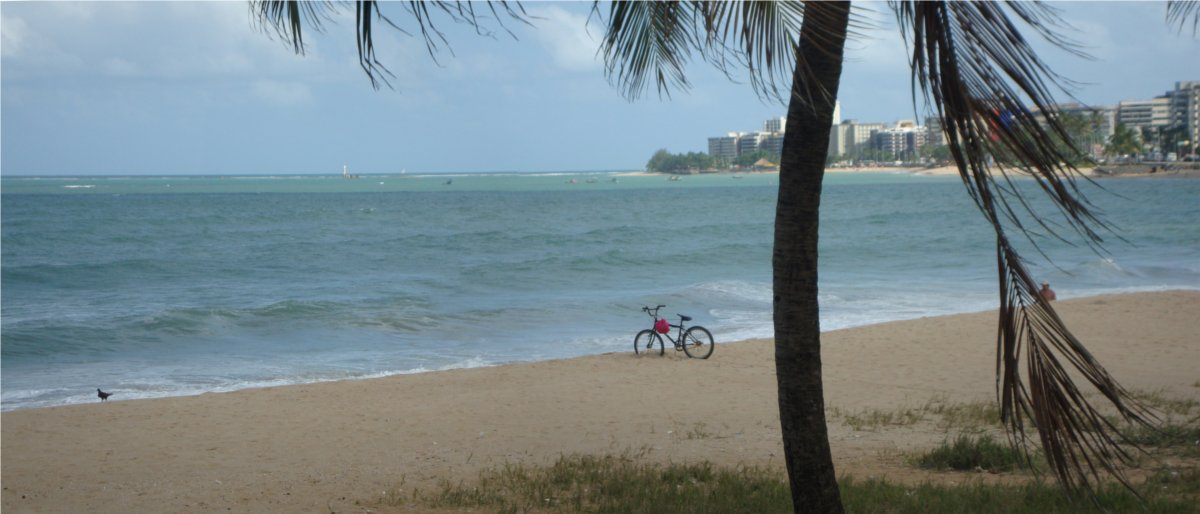
\includegraphics[width=1.1\textwidth]{maceio.jpg}\\
	\tiny{Macei�}
\end{frame}


% ---------------------------------------------------------------------------- %
\section{Segunda se��o}
% ---------------------------------------------------------------------------- %

% ---------------------------------------------------------------------------- %
\subsection{subse��o...}
% ---------------------------------------------------------------------------- %

\begin{frame}
\frametitle{\textbf{Cabe�alho...}}
	\begin{center}
		Texto texto texto texto texto texto texto texto texto texto texto texto texto
		texto texto texto.
	\end{center}
\end{frame}


% ---------------------------------------------------------------------------- %
\section{Algumas considera��es importantes...}
% ---------------------------------------------------------------------------- %

\begin{frame}
\frametitle{Cabe�alho...}
	\begin{enumerate}
    	\item Texto texto texto texto texto texto texto texto...
		\\[0.5em]

    	\item Texto texto texto texto texto texto texto texto...
		\\[0.5em]

		\item Texto texto texto texto texto texto texto texto...
		\\[0.5em]
	\end{enumerate}
\end{frame}



% ---------------------------------------------------------------------------- %
{%\usebackgroundtemplate{}}
\begin{frame}[plain]

	\titlepage

	\addtocounter{framenumber}{-1}
\end{frame}
}

\end{document}
